\documentclass[12pt]{article}

\usepackage{amsmath, amssymb}
\usepackage{graphicx}
\usepackage{gensymb}

\title{The Rendering Equation and Monte Carlo Integration}
\author{Luke Jachimiec}
\date{}

\begin{document}

\maketitle

\begin{abstract}
The rendering equation is one of the foundational mathematical models in modern computer graphics, describing how light is transported and reflected throughout a three-dimensional scene. Its recursive structure allows for the simulation of realistic lighting behaviors such as diffuse reflection, specular reflection, shadows, and global illumination, making it central to physically based rendering and ray tracing. However, because the rendering equation requires integration over infinitely many incoming light directions, obtaining analytical solutions for realistic scenes is generally computationally impossible. As a result, numerical approximation techniques are required.

This paper explores the mathematical structure of the rendering equation and the role of Monte Carlo integration in approximating its solution. The paper begins by introducing the physical interpretation of radiance and the individual terms of the rendering equation. It then examines different material models through Lambertian diffuse reflection and ideal specular reflection using the Dirac delta function, providing analytical examples to demonstrate how reflected radiance is computed in practice. The discussion is extended to multiple incoming light directions and color channel computations to illustrate how realistic lighting behavior emerges from the accumulation of radiance contributions.

The paper then introduces Monte Carlo integration as a method for approximating high-dimensional integrals. Monte Carlo estimators are derived and applied directly to the rendering equation, demonstrating how random sampling can be used to estimate outgoing radiance in complex scenes. Through worked examples, the paper illustrates how Monte Carlo methods enable practical computation of the rendering equation while balancing image quality and computational cost.

\end{abstract}

\section{Introduction}

When it comes to graphics, humans like realism. In computer generated images (CGI), often seen in movies and video games, a lot of the appeal of these movies comes with the ability for a human to feel like what they are seeing is real, like it actually happened on camera. While there are many different ways to tackle this problem, ray tracing is one of the most common practices in developing realistic images. Ray tracing creates hyper realistic images by simulating the physical behavior of light within a scene. It works by tracing the path of light rays shot out by the camera, and calculating how they bounce off, reflect, or refract from objects in a 3D scene to determine the final color and illumination. This is often best seen in the use of reflections, as it algorithmically delivers a realistic real time reflection that would be far too complicated for a human artist to create. But with this realism comes computational cost and complexity.



The first step in simulating the physical light within a scene is developing a way to mathematically model each light ray within the scene. First introduced by James T Kajiya in 1986, the rendering equation provides a mathematical framework that does precisely that. It models the outgoing light at a point as the sum of emitted light and reflected light arriving from every possible direction. Conceptually, the equation captures the behavior of light transport, and is the cornerstone of ray tracing in modern computer graphics.


However, solving the rendering equation is not trivial. Its inherent recursive nature adds computational difficulty, and as the scene complexity increases, the number of possible light paths grows exponentially. Because of this, solving the equation through normal integration and deterministic methods is impossible, thus requiring the use of Monte Carlo integration techniques, which estimate the solution through random sampling rather than exact analytical computation. 

In section 2, we review some simple discrete examples where the rendering equation can be solved by hand to aid in the understanding of the inner workings of the rendering equation. Then in section 3, we present the theory behind Monte Carlo integration, and how it is used to solve the rendering equation in an infinite case, as would typically be seen in practice.







\newpage

\section{The Rendering Equation}
In this section, we present the details of the rendering equation. Although solving the rendering equation is much more difficult than it is displayed in this section, the example problem is defined to offer an intuitive model that can be solved by hand under very specific discrete situations. 

The rendering equation describes the light bouncing through the scene at any given point on a surface. It helps to simulate light reflecting in all directions and light entering from all incoming directions. 
\[
L_o(x,\omega_o) = L_e(x,\omega_o) +
\int_{\Omega} f_r(x,\omega_i,\omega_o)
L_i(x,\omega_i)(\omega_i \cdot n)\, d\omega_i
\]

In this equation, $L_o$ represents the outgoing radiance at point $x$ on a surface in the vector direction $\omega_o$. $L_e$ represents any radiance emitted from the surface itself, such as a billboard or a light source itself. Within the integral along the hemispherical domain $\Omega$, $L_i$ represents the incoming radiance from direction $\omega_i$ towards the point $x$ while $f_r(x, \omega_i, \omega_o)$ is the bidirectional reflectance distribution function, or BRDF, which determines how light is reflected off the surface, dependent on the material properties of the surface.

The integral's domain, defined as the upper hemisphere of directions above the surface, collects only the incoming light arriving from directions above the surface, and light incoming from below the surface contributes nothing to the reflected radiance. The angle of incoming light is captured through $(\omega_i \cdot n)$, or the cosine term, which accounts for the angle between the incoming light direction and the surface normal $n$. This term reduces the contribution of light arriving at angles closer to the surface, and increases contribution of light arriving at angles closer to the surface normal. This process is essential for modeling diffuse reflection. 

\begin{figure}[h] 
    \centering 
    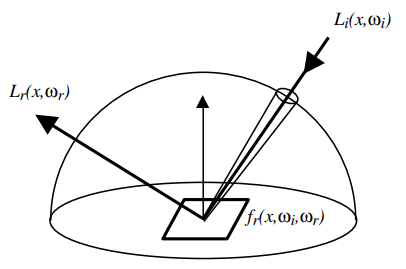
\includegraphics[width=0.35\textwidth]{hemisphere.png} 
    \caption{The hemisphere of incoming light directions} 
\end{figure}

Physically, the equation states that the outgoing light in a given direction comes from two sources: the light produced by the surface itself, and light reflected from the environment. Because the incoming light can come from an infinite number of directions, the equation utilizes an integral rather than a simple sum to account for all incoming directions, but in turn increases its complexity, which makes it difficult to solve analytically in almost all realistic scenes.

The BRDF of the rendering equation also changes depending on the material the light is intersecting with. Different materials react differently to the light, and reflect, refract, or diffuse the outgoing light differently from each other. Three main types of materials often seen are Lambertian or diffuse materials, which diffuse light equally in all directions. Specular reflection or mirror like materials are also common, which only reflect light in a single reflected direction, and dielectric materials, such as glass or water, that refract light through the object, as well as reflect it. In this paper, we will explore Lambertian and reflective materials.


\subsection{Lambertian Reflection}
Lambertian reflection describes an ideal diffuse surface that scatters incoming light equally in all outgoing directions. Common examples of this type of surface include matte surfaces, such as cardboard and walls.

Since it is a type of material, Lambertian reflection relies on a specifically defined BRDF function. For a perfectly ideal Lambertian surface, the BRDF is constant, with an albedo or reflectency property of $\rho$:
\[f_r = \frac{\rho}{\pi}\]




Look at the nearest wall. Given that it is a solid matte color and reletively well lit, if you were to change your position and walk around your room staring at the same spot, the overal radiance and color of that spot would not change no matter how you move. Because of this, the BRDF of a Lambertian surface does not depend on direction. The amount of reflected light is determined only by the incoming light and the angle between that light and the surface normal, completely ignoring where the observer is positioned. \newline
\newpage
Substituting this in into the rendering equation gives

\[
L_o(x, \omega_o) = L_e(x, \omega_o) + \int_{\Omega}\frac{\rho}{\pi}L_i(x, \omega_i)(\omega_i\cdot n) d\omega_i
\]

For a diffuse surface, light arriving straight on contributes more light than shallow angles, due to the cosine term being closer to zero when it becomes closer to perpendicular. So Lambertian surfaces appear brightest when illuminated head and dimmer towards the edges of the lit regions. 
\newline

In a simple one-ray example, if a single incoming light direction $\omega_i$ strikes a surface point with normal $n$, the reflected outgoing radiance is proportional to the incoming radiance, the albedo, and the cosine of the angle between light and surface normal. 

For example, with incoming radiance of 10, at an angle of 45 degrees from the normal and an albedo of 0.8, the rendering equation becomes 
\[
L_o(x, \omega_o) = \frac{0.8}{\pi} \cdot 10 \cdot cos(45)
\]

This evaluates to $L_o = 1.8$, since there is no emitted radiance, $L_e = 0$.
\\\\
In basic terms, this means that of the 10 units of radiance entering the scene from a direction, only 1.8 units of radiance is exiting the scene in any given direction. No matter where the observer is positioned, the value will always be the same, since the $\omega_o$ term does not appear anywhere in the equation for Lambertian reflection.


\subsection{Radiance and Color Channels}

Radiance is defined to be the physical measure of light passing through or emitted from a surface, defined as radiant power per unit solid angle per unit projected source area, which is measured mathematically as watts per square meter per steradian ($W \cdot m^{-2} \cdot sr^{-1}$). Steradians are the units for solid angles. Steradians are unitless, as they are often seen as a projection of an object onto a unit sphere, and the projection is the solid angle of the object as viewed from the center of the sphere.

The rendering equation utilized radiance to describe both the incoming light arriving at a surface, as well as the outgoing light that leaves the surface towards the viewer. Unlike in our previous example in 2.1, light is not represented as a single scalar value. Instead, radiance is evaluated per wavelength. In practice, most rendering systems approximate this by representing radiance as a three-component vector corresponding to red, green, and blue color channels:   
\[
L = (R, G, B)
\]
Because of this representation, the rendering equation must be evaluated independently for each color channel. 
\newline\newline
Consider a diffuse surface with albedo 
\[
\rho = (0.8, 0.1, 0.1)
\]
which represents a surface that reflects mostly red light, and only a small amount of green and blue light. Like before, Lambertian BRDF is given by 
\[
f_r = \frac{\rho}{\pi}
\]
and suppose a white light source strikes the surface with incoming radiance 
\[
L_i = (10,10,10)
\]
at an angle of \(45^\circ\) and a solid angle \(\Delta\omega = 1\), the outgoing radiance can be computed per color channel using the rendering equation 
\[
L_o = f_r \cdot L_i \cdot (\omega_i \cdot n) \cdot \Delta\omega
\]
Substituting the values gives

\[
L_o = (1.8, 0.23, 0.23)
\]
indicating the reflected light is a strong red, as expected from the albedo values. Like our previous example in 2.1, the outgoing radiance of the red color channel is the same 1.8 as before, but the green and blue channels reflect less light.

Similarly, using the same surface, but now with an incoming light that is purely blue 
\[
L_i = (0,0,10)
\]

Since the surface reflects very little blue light, as defined the albedo $\rho$, and the red and green channels receive no incoming energy, the resulting outgoing radiance, when calculated like before, is 

\[
L_o = (0,0,0.23)
\]
illustrating how material properties influence the color of reflected light. Surfaces that selectively absorb and reflect different amounts of each wavelength of light react differently to the light source, and can drastically change the outgoing radiance and the final color observed by the viewer. Different materials entirely may offer a completely different method of computing the outgoing light, and thus a completely different behavior all together.

\subsection{Specular Reflection and the Dirac Delta Function}

Ideal specular reflection models perfectly smooth mirror-like surfaces, where all incoming radiance from a single direction is reflected into a single outgoing direction. Unlike diffuse reflection, which distributes energy over a hemisphere, ideal specular reflection concentrates all reflected energy along a single deterministic direction.
\newline

An ideal mirror surface does not scatter any of the incoming light. The outgoing direction is fully determined by the law of reflection:
\[
\omega_r = 2(\omega_i \cdot n)n - \omega_i,
\]
where \( \omega_i \) is the incident direction, \( \omega_r \) is the reflected direction, and \( n \) is the surface normal.


For a given incident direction \( \omega_i \), the reflected direction \( \omega_r \) is unique. This determinism implies that the BRDF must concentrate all reflected energy at a single outgoing direction.
\newline

The ideal specular BRDF can be expressed using the Dirac delta distribution:
\[
f_r(\omega_i, \omega_o) = \rho \, \delta(\omega_o - \omega_r),
\]
where \( \rho \) is the reflectance coefficient and \( \delta \) is the Dirac delta function defined over the unit hemisphere.

This formulation encodes the fact that reflection occurs only when \( \omega_o = \omega_r \), and is zero elsewhere.
\newpage
Given the rendering equation:
\[
L_o(x, \omega_o) = L_e(x, \omega_o) + \int_{\Omega} f_r(x, \omega_i, \omega_o)\, L_i(x, \omega_i)\, (\omega_i \cdot n)\, d\omega_i.
\]
Substituting the delta-based BRDF yields:
\[
L_o(x, \omega_o) = L_e(x, \omega_o) + \int_{\Omega} \rho \, \delta(\omega_o - \omega_r)\, L_i(x, \omega_i)\, (\omega_i \cdot n)\, d\omega_i.
\]
Using the sifting property of the Dirac delta function:
\[
\int f(x)\,\delta(x - x_0)\,dx = f(x_0),
\]
the integral collapses to:
\[
L_o(x, \omega_o) = L_e(x, \omega_o) + \rho \, L_i(x, \omega_r)\, (\omega_r \cdot n).
\]
Thus, instead of integrating over all incoming directions, only the single reflected direction contributes to the outgoing radiance.
\newline

Now, consider a simple scene consisting of an ideal mirror surface with normal \( n = (0,0,1) \), illuminated by a single directional light source. The incoming light arrives from direction
\[
\omega_i = \left(\frac{1}{\sqrt{2}}, 0, \frac{1}{\sqrt{2}}\right),
\]
i.e., at a $45^\circ$ angle from the surface normal.\newline
The incident radiance is constant and given by:
\[
L_i(\omega_i) = (10, 10, 10),
\]
in RGB radiance units.
Using the law of reflection:
\[
\omega_r = 2(\omega_i \cdot n)n - \omega_i,
\]
we compute:
\[
\omega_i \cdot n = \frac{1}{\sqrt{2}},
\]
thus:
\[
\omega_r = 2\left(\frac{1}{\sqrt{2}}\right)(0,0,1) - \left(\frac{1}{\sqrt{2}}, 0, \frac{1}{\sqrt{2}}\right),
\]
which simplifies to:
\[
\omega_r = \left(-\frac{1}{\sqrt{2}}, 0, \frac{1}{\sqrt{2}}\right).
\]

\begin{figure}[h]
    \centering
    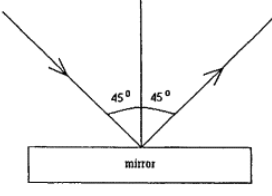
\includegraphics[width=0.25\textwidth]{specular_reflection.png}
    \caption{Angle of perfect reflection}
\end{figure}

The angle of perfect reflection $\omega_r$ is 45 degrees from the normal, as seen in figure 2 above. 

Let the specular reflectance be wavelength-dependent:
\[
\rho = (0.8, 0.1, 0.1),
\]
indicating a surface that strongly reflects red light while heavily attenuating green and blue components.
Using the ideal specular BRDF:
\[
f_r(\omega_i, \omega_o) = \rho \, \delta(\omega_o - \omega_r),
\]
the rendering equation collapses to:
\[
L_o(\omega_o) = \rho \, L_i(\omega_i)\, (\omega_i \cdot n)
\quad \text{when } \omega_o = \omega_r.
\]
Substituting values:
\[
(\omega_i \cdot n) = \frac{1}{\sqrt{2}}, \quad L_i = (10,10,10),
\]
we obtain component-wise multiplication per color channel:
\[
L_o(\omega_r) = (0.8, 0.1, 0.1) \cdot (10, 10, 10) \cdot \frac{1}{\sqrt{2}},
\]
Thus, the outgoing radiance is:
\[
L_o(\omega_r) =
\left(
\frac{0.8\cdot10}{\sqrt{2}},
\frac{0.1\cdot10}{\sqrt{2}},
\frac{0.1\cdot10}{\sqrt{2}}
\right)
\]
So
\[
L_o(\omega_r) =
\left(
\frac{8}{\sqrt{2}},
\frac{1}{\sqrt{2}},
\frac{1}{\sqrt{2}}
\right),
\]
and zero for all other directions due to the Dirac delta constraint:
\[
L_o(\omega_o) = 0 \quad \text{for } \omega_o \neq \omega_r.
\]
The fact that $L_o = 0$ for all other directions reinforces the fact that moving the camera from the perfect reflected direction will prevent the camera from receiving the outgoing light reflected by the mirror, thus getting no reflected light, as there is only one incoming light ray. 

This can be visualized with a mirror in real life, where moving around a mirror while focusing on the same physical position on the mirror will change what is seen at that point on the mirror, reinforcing the idea that the camera must be at the correct $\omega_r$ angle to be seen

In real life, however, no mirror is truly perfect and consists of many micro roughness, which causes some diffuse properties, but in computer simulations, this can be ignored, as it can be defined and simulated to be perfect without the need to have microscopic inconsistencies in the mirror's surface. 


\subsection{Multiple Incoming Light Directions}

In realistic lighting scenarios, a surface is very rarely illuminated by a single incoming light direction. Instead, light arrives from an infinite number of possible directions across a hemisphere above the surface. Each of these incoming light directions contributes to the outgoing radiance, increasing both the complexity and realism of the resulting image. 

Extending the rendering equation to a discrete finite number of incoming light directions, we can approximate the integral as a finite sum:

\[
L_o \approx \sum_{k=1}^{N} f_r \, L_i(\omega_k) \, (\omega_k \cdot n) \, \Delta \omega_k
\]
where each direction $\omega_k$ represents a sampled incoming light ray.
\newline

Consider a diffuse surface with albedo $\rho = 0.8$, and two light rays arriving at point $x$ at $45 \degree$ and $30 \degree$ from the normal, both of which have a $L_i = 10$.
In 2.1.1, we have already computed $L_o$ at $45 \degree$ before to be 1.8, and doing the same calculation for $30 \degree$ yields an $L_o = 2.2$. Summing these two samples yields an outgoing radiance of $L_o = 4$, as more light hitting the same point contributes more radiance to the scene.

It is intuitive that this can process be done without constant values within each color channel but has been left out for simplicity.
\newline



For any finite number of rays, the outgoing radiance can be calculated through the summing of individual rays for each direction sample.
\newline

Consider a diffuse surface with albedo $\rho = (0.8, 0.8, 0.8)$ and 10 incoming rays from various directions, as defined in table 1:
\begin{table}[h!]
\centering
\begin{tabular}{|c|c|c|c|c|}
\hline
\textbf{Ray \#} & \textbf{Angle $(\theta)$} & \textbf{$\cos(\theta)$} & \textbf{Radiance $L_i$} & \textbf{Color} \\
\hline
1  & 0   & 1.000 & $(10,10,10)$ & White \\
2  & 30  & 0.866 & $(10,10,10)$ & White \\
3  & 45  & 0.707 & $(10,10,10)$ & White \\
4  & 60  & 0.500 & $(10,10,10)$ & White \\
5  & 75  & 0.259 & $(10,0,0)$ & Red \\
6  & 30  & 0.866 & $(0,10,0)$ & Green \\
7  & 45  & 0.707 & $(0,0,10)$ & Blue \\
8  & 60  & 0.500 & $(10,10,0)$ & Yellow \\
9  & 0   & 1.000 & $(0,10,10)$ & Cyan \\
10 & 90  & 0.000 & $(10,0,10)$ & Purple \\
\hline

\end{tabular}
\caption{Table of incoming light rays within a scene}
\end{table}

\newpage
The contribution of each ray can be computed independently and accumulated per color channel. Before applying the BRDF function, we can calculate

\[
\begin{aligned}
R &= \sum_{i=1}^{10} L_i \cos(\theta) = 38.32 \\
G &= \sum_{i=1}^{10} L_i \cos(\theta) = 54.39 \\
B &= \sum_{i=1}^{10} L_i \cos(\theta) = 47.80
\end{aligned}
\]


\begin{align*}
R &= 10(1) + 10(0.866) + 10(0.707) + 10(0.5) + 10(0.259) \\
  &\quad + 0 + 0 + 10(0.5) + 0 + 10(0) \\
  &= 10 + 8.66 + 7.07 + 5 + 2.59 + 5 \\
  &= 38.32
\end{align*}

\begin{align*}
G &= 10(1) + 10(0.866) + 10(0.707) + 10(0.5) \\
  &\quad + 0 + 10(0.866) + 0 + 10(0.5) + 10(1) + 0 \\
  &= 10 + 8.66 + 7.07 + 5 + 8.66 + 5 + 10 \\
  &= 54.39
\end{align*}

\begin{align*}
B &= 10(1) + 10(0.866) + 10(0.707) + 10(0.5) \\
  &\quad + 0 + 0 + 10(0.707) + 0 + 10(1) + 10(0) \\
  &= 10 + 8.66 + 7.07 + 5 + 7.07 + 10 \\
  &= 47.80
\end{align*}
Thus, the accumulated radiance across channels is
\[
(R, G, B) = (38.32,\; 54.39,\; 47.80).
\]
Scaling by the Lambertian BRDF,
\[
f_r = \frac{\rho}{\pi} = \frac{0.8}{\pi} \approx 0.2546,
\]
we obtain
\begin{align*}
L_o
& \approx (38.32,\; 54.39,\; 47.80)\, \cdot f_r \\
& \approx (38.32,\; 54.39,\; 47.80)\,\cdot(0.2546) \\
&\approx (9.76,\; 13.84,\; 12.17).
\end{align*}

This can be done for any finite number of light samples as well as extended to reflective surfaces.
\newline



While summation works for a small number of rays, real-world scenes involve infinetly many incoming directions, thus an infinite number of samples. As the number of light interactions increases, direct computation becomes impractical and slow, thus motivating the use of other stochastic approximation methods.



\section{Monte Carlo Integration}

Monte Carlo integration provides a numerical method for approximating integrals using random sampling. It is particularly useful when dealing with high-dimensional integrals, such as the rendering equation. In general, Monte Carlo integration is not limited to only high dimensional integrals or the rendering equation. Any integral of the proper form can be estimated using Monte Carlo integration, through most low dimension integrals do not see any benefit compared to normal analytical integration methods. 
\newline

Suppose we want to compute an integral on domain $\Omega$.
Given an integral of the form
\[
I = \int_\Omega f(x)\,dx
\]
we pick a Probability Density Function $p(x)$ where 
\[
p(x) \geq 0 \ and \int_\Omega p(x)\,dx = 1
\]
Multiplying and dividing the integrand by $p(x)$ gives us 
\[
I = \int_\Omega f(x)\,dx = \int_\Omega \frac{f(x)}{p(x)}p(x)\,dx
\]
In probability theory, by definition, the expected value $\mathbb{E}[g(X)] = \int_\Omega g(x)p(x)dx$.
Using this fact, we see that since 
\[
I  = \int_\Omega \frac{f(x)}{p(x)}p(x)\,dx
\]
then it follows that
\[
I = \mathbb{E}\left[\frac{f(x)}{p(x)}\right]
\]
and since the expected value of a random variable can be approximated by the sample average, we can draw $N$ random samples $x_i$ from $p(x)$ to get out Monte Carlo Estimator.
\[
I \approx \frac{1}{N}\sum_{i=1}^N \frac{f(x_i)}{p(x_i)} 
\]
This approximation works for any integral of the form $I = \int f(x)dx$.
\newline
For example:
\newline
Consider the integral over the unit square:
\[
I = \int_0^1 \int_0^1 (x^2 + y^2)\, dx\, dy.
\]

Using Monte Carlo integration, we sample $N$ points $(x_i, y_i)$ uniformly
from $[0,1]^2$ and estimate:

\[
I \approx \frac{1}{N} \sum_{i=1}^{N} \frac{(x_i^2 + y_i^2)}{p(x_i)}.
\]
Through uniform sampling, we obtain a PDF $p(x,y) = 1\ for\ (x,y) \in [0,1]^2$.
Thus $I = \mathbb{E}[f(x,y)]$ trivially.
\newline
Now, using $N = 5$ ``random" samples:
\[
(0.2,0.5),\ (0.7,0.1),\ (0.4,0.9),\ (0.8,0.3),\ (0.6,0.6),
\]
we compute:
\[
I \approx \frac{1}{5}(0.29 + 0.50 + 0.97 + 0.73 + 0.72) = 0.642.
\]
The exact value is:
\[
I = \frac{2}{3} \approx 0.6667.
\]
Choosing more samples of $N$ would let the approximation of $I$ approach the expected result, thus showing how Monte Carlo integration can be used to approximate and evaluate any integral. The estimated value and convergence rate can differ based on the sampling strategy used. In rendering, the common sampling techniques consist of Uniform Hemisphere Sampling and Cosine-Weighted Sampling.

\subsection{Sampling Strategies}
The choice of probability density function $p(x)$ plays a critical role in the efficiency and accuracy of Monte Carlo estimation. Picking a PDF can change not only the estimated value, but also increase or decrease the convergence rate to the expected value. While some PDFs are more beneficial than others, it greatly depends on the goal of the Monte Carlo Estimator, and what you are trying to accomplish.

For rendering, the two most common and useful sampling strategies are Uniform Hemisphere Sampling and Cosine-Weighted Sampling.

\subsubsection{Uniform Hemisphere Sampling}

In uniform sampling, each possible sample has equal probability of being chosen. 
In rendering, this means that each direction within the hemisphere has the same probability to  be chosen as any other direction, thus given equal chance and full spread of directions being sampled. 

It can be seen that the probability density function of uniform hemisphere sampling is constant: 
\[
p(\omega) = \frac{1}{2\pi}
\]

This approach is simple to implement, but is relatively inefficient, and does not obtain a full optimized sampling strategy, as it does not account for the angle of incidence, thus missing directions that are seen as more important or less important to the final outgoing radiance. \newline
\textbf{Advantages:}
\begin{itemize}
\item Simple and straightforward concept and implementation.
\item Uniform coverage of hemisphere ensures no direction will be left out.
\item Generating samples is fast and requires low computational overhead.

\end{itemize}
\textbf{Disadvantages:}
\begin{itemize}
\item High variance as samples near the horizon $(90 \degree)$ contribute little light, requiring more samples to achieve full image coverage.
\item Inefficient sampling of important directions since it does not account for angle of incidence.
\item Though rare, uniform samples can sometimes cluster together, leading to visible artifacts in the final render.
\end{itemize}

\subsubsection{Cosine-Weighted Sampling}
Cosine weighted sampling improves efficiency by sampling directions proportional to the cosine term, with PDF:

\[
p(\omega) = \frac{\cos(\theta)}{\pi}
\]

This aligns the sampling distribution with the integrand of the rendering equation, reducing variance. As we will see later, using this sampling strategy allows for some cancellation to occur in the Monte Carlo estimator, which helps cosine-weighted sampling to be widely used in rendering.
\newline
\textbf{Advantages:}
\begin{itemize}
\item Lower variance since only important rays and directions will be sampled.
\item More efficient convergence since less time will be spent on insignificant directions.
\end{itemize}
\textbf{Disadvantages:}
\begin{itemize}
\item Slightly more complex implementation as more complex methods need to be used.
\end{itemize}

\newpage
\subsection{Monte Carlo Estimation in Rendering}

When applying Monte Carlo integration to the rendering equation as in 3.1.1, we take our generalized Monte Carlo Estimator 
\[
I \approx \frac{1}{N}\sum_{i=1}^N \frac{f(x_i)}{p(x_i)}
\]
and thus obtain the Monte Carlo estimator for the Rendering Equation to be:
\[
L_o(x, \omega_o) \approx \frac{1}{N} \sum_{i=1}^{N}
\frac{f_r(x,\omega_i,\omega_o)\,L_i(x,\omega_i)\,(\omega_i \cdot n)}{p(\omega_i)}
\]
with each sample $\omega_i$ being a randomly chosen incoming light direction.

Given a scene with a lambertian surface with albedo 0.8
assume the lighting consists of two main elements:
\textbf{Sky:} Upper hemisphere where $L_i(\omega) = (2,4,8)$
\textbf{Sun:} A bright disk centered at $(\frac{\sqrt{2}}{2}, 0, \frac{\sqrt{2}}{2})$ and $L_i(\omega) = (30,30,30)$ within a $5\degree$ from the center.

\begin{figure}[h]
    \centering
    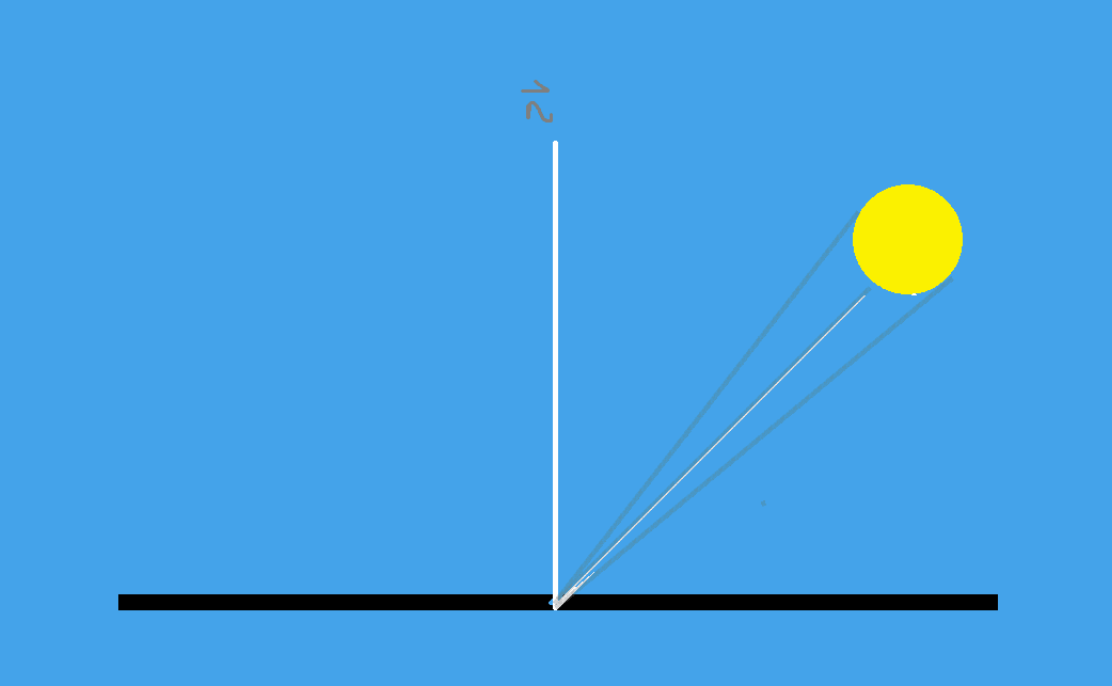
\includegraphics[width=0.40\linewidth]{MonteCarloExample.png}
\end{figure}
Take the rendering equation and substitute BRDF
\[
L_o = \int_{\Omega} \frac{0.8}{\pi}\, L_i(\omega_i)\, (\omega_i \cdot n)\, d\omega_i
\]
Using cosine-weighted hemisphere sampling, define the PDF as
\[
p(\omega) = \frac{\cos \theta}{\pi}
\]
Thus, the Monte Carlo estimator becomes
\[
L_o \approx \frac{1}{N} \sum_{i=1}^{N}
\frac{\frac{0.8}{\pi}\, L_i(\omega_i)\, (\omega_i \cdot n)}
{\frac{\cos \theta_i}{\pi}}
\]
And by cancellation of terms, we get
\[
L_o \approx \frac{1}{N} \sum_{i=1}^{N} 0.8\, L_i(\omega_i)
\]
Now we are able to pick $N$ random direction samples $\omega$, sum up and average their corresponding radiance values, and estimate the outgoing radiance from the point on the surface. So, if we were to pick, for example, 10 random samples as defined by table 2:
\begin{table}[h]
\centering
\begin{tabular}{|c|c|c|c|}
\hline
Ray & Angle & Hit Sun? & $L_i$ \\ \hline
1  & 10° & no  & (2,4,8) \\ \hline
2  & 20° & no  & (2,4,8) \\ \hline
3  & 40° & yes & (30,30,20) \\ \hline
4  & 60° & no  & (2,4,8) \\ \hline
5  & 30° & no  & (2,4,8) \\ \hline
6  & 50° & yes & (30,30,20) \\ \hline
7  & 70° & no  & (2,4,8) \\ \hline
8  & 25° & no  & (2,4,8) \\ \hline
9  & 15° & no  & (2,4,8) \\ \hline
10 & 45° & yes & (30,30,20) \\ \hline
\end{tabular}
\caption{Table of ``randomly" selected directions}
\end{table}

As done in section 2.4, it can be intuitively seen that the sum of incoming light for this example yields
\[L_i = (104, 114, 116)\]
After averaging by $N$ \[
\left(\frac{104}{10}, \frac{114}{10}, \frac{116}{10}\right)
=
(10.4, 11.4, 11.6)
\]
Now applying the BRDF 
\[
L_o \approx (10.4, 11.4, 11.6) \cdot 0.8 = (8.32, 9.12, 9.28)
\]
Adding more samples will increase the accuracy of your prediction, and will eventually converge to the actual expected value of $L_o$

\newpage
\subsection{Convergence and Image Quality}
Monte Carlo estimators converge at a rate of:
\[
O\left(\frac{1}{\sqrt{N}}\right)
\]

This means that increasing the number of samples $N$ improves the accuracy, but adds complexity and computation time. Low sample counts will produce noisy results, as there is not enough samples of rays to fully populate the scene, and thus not allowing full coverage or accurate results. High sample counts produce smoother, more accurate images, but the computational cost increases with the number of samples. In practice, a hard cut off of the number of samples is used and the estimation is deemed "good enough" at a point where increasing samples does not help improve the image quality.

In rendering, this trade off between computational cost and image quality is a central element, as efficiency is of high importance in advanced rendering, and thus needs to be fast without decreasing the overall image quality.  

\begin{figure}[h]
    \centering
    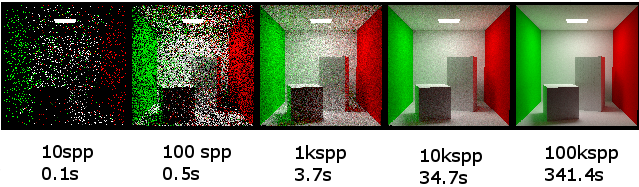
\includegraphics[width=1\textwidth]{SPP.png}
    \caption{As samples increase, image quality increases}
\end{figure}

As shown in Figure 3, a low number of sampled rays creates a noisy incomplete image, but is rendered very quickly. A high number of samples creates a smoother image with almost no noticeable noise, but takes much longer to render.

\newpage
\section{Conclusion}

Despite its conceptual simplicity, the rendering equation presents a large computational challenge due to its recursive structure and high-dimensional integration domain. Realistic scenes contain infinitely many possible light interactions, as well as requiring the rendering equation evaluation for every ray object intersection happening within the scene.  This makes direct analytical evaluation impractical in nearly all applications.

In practical real time rendering, ray tracing is accompanied by many other rendering techniques in order to speed up the process of rendering and ray tracing as a whole. Ray tracing an entire scene without the use of any of the other techniques can quickly become too overwhelming and cause massive delays in production and efficiency. While it does provide the best quality of images, the amount of time and computing power required alone is enough to not be a practical method of rendering a scene, but is still used as a ``finishing touch" to squeeze out some extra quality or increase the realism of reflections. In video games, graphics processing units (GPUs) have developed dedicated hardware specifically made for ray tracing, which allows faster computation and rendering of ray tracing algorithms, which helps to deliver render times as low as $\frac{1}{120}$th of a second, in order to achieve 120 frames per second in gaming. 

As research and hardware improve, ray tracing is only getting faster and faster, but the core principles have remained the same for years, and have no plans of changing anytime soon. Mathematically, ray tracing is at its peak performance, and it is up to the hardware and code in order to optimize the algorithms to achieve faster render times.

While the beginning of this project posed some challenges on the overall scope, vision, and goals of the project, I believe that I was able to develop a solid foundation and understanding of the project and topics introduced. I can confidently say that I have learned something new, and gained enough understanding to call myself proficient in the topic. Although there is still more to be learned and researched, I believe that the amount of work fell within the scope of this semester of research, and left me with all I could realistically ask for given this short amount of time. 

Overall, this project provided a deeper insight into the inner workings of graphics rendering, and was able to help develop my understanding as a whole. Alongside my Computer Science capstone project, where I implemented the ideas of the rendering equation and Monte Carlo integration to develop a ray tracing algorithm and pipeline to render $.obj$ files and turn them into full ray traced scenes and images. Working simultaneously on the rendering equation and the computer science program helped join the ideas together, and gain a better understanding of how models like this are implemented in practice.





\newpage

\section{Bibliography}
\begin{itemize}
    
    \item Kajiya, James T. \textit{The rendering equation.} ACM SIGGRAPH Computer Graphics, vol. 20, no. 4, 31 Aug. 1986, pp. 143–150,
    \item Pharr, Matt, Jakob, Wenzel, and Humphreys, Greg. \textit{Physically Based Rendering}. 3rd ed., 2016.
    \item Dutré, Philip. \textit{Global Illumination Compendium}, 2003.
    \item Shirley, Peter. \textit{Fundamentals of Computer Graphics}. CRC Press.
    \item Shirley, Peter. \textit{Ray Tracing in One Weekend.} Ray Tracing in One Weekend Series, raytracing.github.io/books/RayTracingInOneWeekend.html. Accessed 1 Dec. 2025. 
    \item Veach, Eric. \textit{Robust Monte Carlo Methods for Light Transport Simulation}. Stanford University, Dept. of Computer Science, 1998. 
    \item Chapter 1 Monte Carlo Path Tracing, graphics.stanford.edu/courses/cs348b-01/course29.hanrahan.pdf. Accessed 2 Dec. 2025. 
    \item Wolfe, Alan. “Path Tracing – Getting Started With Diffuse and Emissive.” Demofox.Org, https://blog.demofox.org/2016/09/21/path-tracing-getting-started-with-diffuse-and-emissive/. Accessed 13 May 2026. 
    \item Moller et al. \textit{Real-Time Rendering}. CRC Press, 2019. 
    \item Dunn, Ian. \textit{Graphics Programming Compendium.} Graphics Compendium, graphicscompendium.com/index.html. Accessed 1 Dec. 2025. 
    \item Shirley, P., Wang, C., and Zimmerman, K. Monte carlo techniques
for direct lighting calculation. ACM Transactions on Graphics 15 (09
1999)
    \item Zimmerman, K. Developing the Rendering Equations. Princeton Uni-
versity
    \item Novák, Jan, et al. “Monte Carlo methods for Volumetric Light Transport Simulation.” Computer Graphics Forum, vol. 37, no. 2, May 2018, pp. 551–576, https://doi.org/10.1111/cgf.13383. 
    \item Arvo, James. “Analytic methods for simulated light transport.” (1995).
    
\end{itemize}



\end{document}